\chapter{Verteilungssicht}

\begin{figure}[h!]
	\centering
	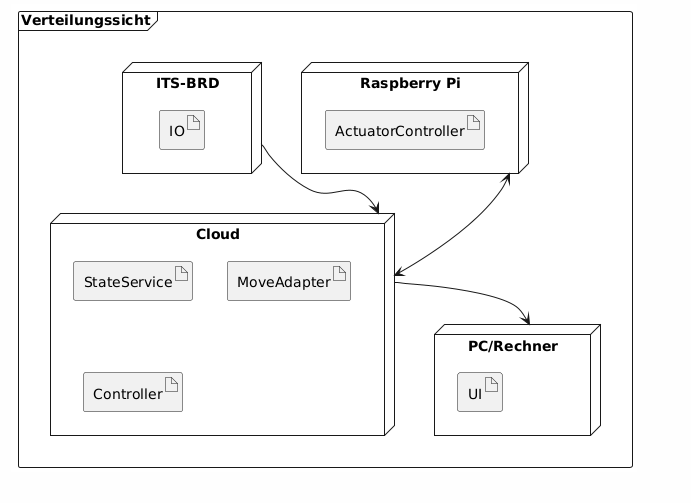
\includegraphics[scale=.5]{diagrams/deploymentView.png}
	\caption{Deployment Diagramm (Produtiv)}
	\label{fig:deployment-prod-grafik}
\end{figure}

% Notizen zu https://docs.arc42.org/section-7/

% - Geografische Orte
% - Umgebungen (dev / test / prod / temporary or ephemeral)
% - Computers (entwickler laptop/labor-pc/roboter+rasPi/ITS-board/ICC/VMs oder Container?)

% - Kein plan: Processorcs, channels, net topologies 
%   Rede ist auch manchmal von Arc42 für Hardware Desing, nehme an Processors ist also latte.
% - Mapping von Software (5. Building blocks) auf infrastruktur
% - Wir muessen nur Infrastruktur dokumentieren die für Software notwendig ist.

% Maybe the highest level deployment diagram is already contained in section 3.2. as technical context with your own 
% infrastructure as ONE black box. In this section you will zoom into this black box using additional deployment 
% diagrams.

% UML Wenn infrstruktur einigermassen komplex

% Hardware anforderungen (bspw. Java umgebung für entwickle laptop)

% Aus https://docs.arc42.org/tips/7-1/
% Weitere Hardware wie Switch/Router

% Aus https://docs.arc42.org/tips/7-2/
% If hardware plays an important role in the architecture, you can even use a node-template for that purpose, 
% similar to the following table:
% Node <node-name>
% | Responsibility	            | what is the role of this hardware element, what’s it doing?               |
% | (technical) characteristics	| i.e. nr of cpus/cores, memory, throughput, nr-of-ports, vendor, model…    |
% | associated building blocks 	| what part of the software is running on this hardware?                    |
% | reason for selection	    | why was this particular hardware selected?                                |

% https://docs.arc42.org/tips/7-3/ | Hierarchisch immer detaillierter UML standard(?) "O-O Notation"
% https://docs.arc42.org/tips/7-4/ | Hierarchisch immer detaillierter nur anders (nicht UML glaub ich)
% https://docs.arc42.org/tips/7-5/ | Mapping Building Blocks auf Hardwareumgebung(en)
% https://docs.arc42.org/tips/7-6/ | UML Hardware/Building Blocks
% https://docs.arc42.org/tips/7-7/ | Tabelle statt UML (aber auch UML)
% gibt noch 3 weitere tipps goaub ich...

% 7.1 Infrastructure Level 1

% Describe (usually in a combination of diagrams, tables, and text):

% the distribution of your system to multiple locations, environments, computers, processors, .. as well as the physical connections between them
% important justification or motivation for this deployment structure
% Quality and/or performance features of the infrastructure
% the mapping of software artifacts (building blocks) to elements of the infrastructure
% For multiple environments or alternative deployments please copy that section of arc42 for all relevant environments. **

% < insert infrastructure overview diagram >

% Motivation
% < insert description of motivation or explanation in text form>

% (optional) Quality and/or Performance Features
% < optionally insert description quality or performance features >

% Mapping
% < insert description of mapping of building blocks >

% 7.2 Infrastructure Level 2
% Here you can include the internal structure of (some) infrastructure elements from infrastructure level 1.
% Please copy the structure from level 1 for each selected element.

% 7.2.1 < Infrastructure element 1>
% < insert diagram + explanation >

% 7.2.2 < Infrastructure element 1>
% < insert diagram + explanation >

% …
% < insert diagram + explanation >

% 7.2.n < Infrastructure element 1>
% < insert diagram + explanation >